\onehalfspacing
%% SECTION
\section{Project Research Plan}

The figure \ref{fig:gantt} show a Gantt Diagram with the initial planning of the project.
It is divided in the following milestones needed to the accomplishment of the project:

\begin{itemize}
    \item \textbf{Definition and planning:} this milestone consists on the definition of the project and its planning.
    \item \textbf{State of the art:} to accomplish this milestone, a deep study on the recent activities in the field will be done.
    \item \textbf{Design and implementation:} during this stage, the implementation of the study will be carried on.
    \item \textbf{Write the report:} once the previous step is finish, a report explaining the results must be written.
    \item \textbf{Thesis defense:} a presentation of the current work must be done to accomplish this milestone.
    \item \textbf{Public presentation:} as a last step, the work must be publicly presented to an academic trial.
\end{itemize}

An extra column has been added to the Gantt diagram to illustrate the relation between the milestones and the corresponding phase or phases of a CRISP-DM project.

\begin{figure}[h]
    \centering
    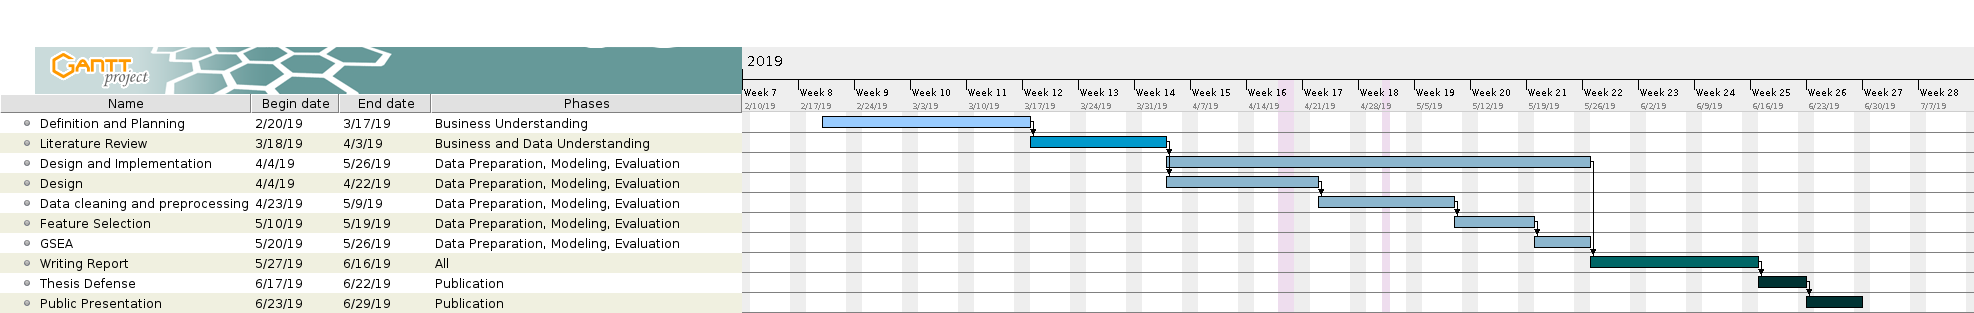
\includegraphics[angle=90, width=\textwidth,height=\textheight,keepaspectratio]{../figs/TFM_plan.png}
    \caption{Gantt Project}
    \label{fig:gantt}
\end{figure}